\section{Einteilung \& Design}
\setauthor{David Altenhofer}
Sobald die Festlegung und die Aufteilung der Arbeitspakete in der Firma geregelt waren, wurde mit dem Use-Case-Diagramm begonnen.
Es haben sich alle Teamkollegen der Diplomarbeit daran beteiligt und nach einigen Änderungen, Diskussionen und Empfehlungen 
war das Use-Case-Diagramm nach zwei Tagen finalisiert.
\\
\\
\\

\begin{figure}[ht!]
    \centering
    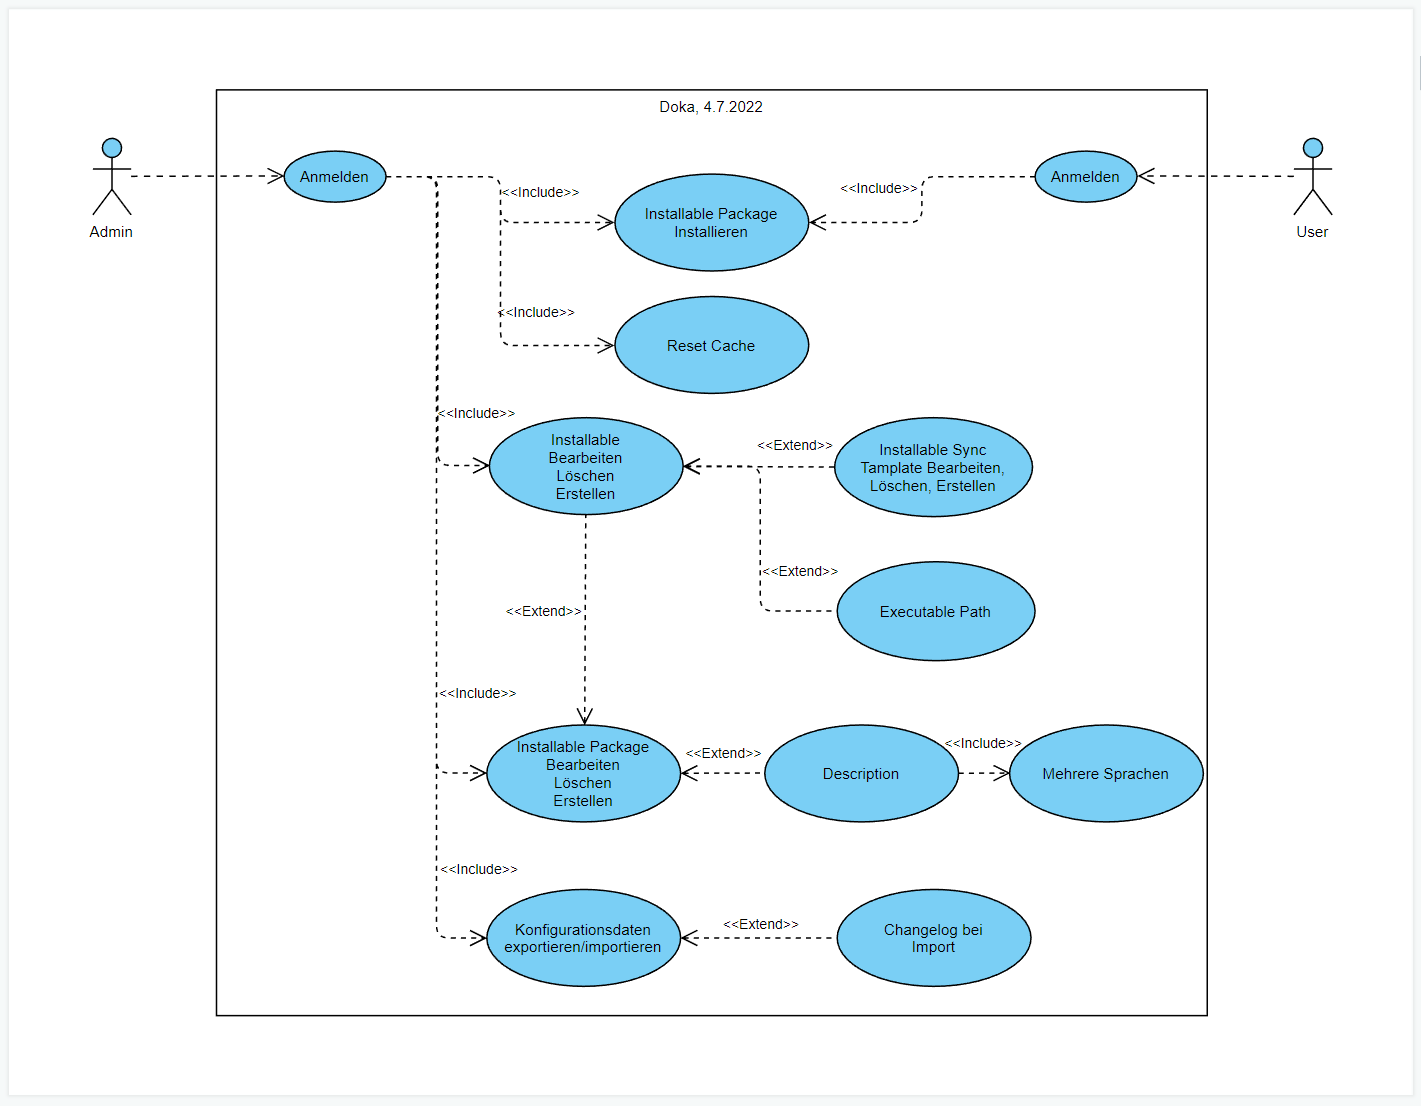
\includegraphics[scale=0.3]{pics/UCD.png}
    \caption{\label{fig:The-caption}Use-Case-Diagramm \cite{APCW2006}}
    \label{fig:impl:use-case-diagramm}
  \end{figure}
\newpage

  Ein Use-Case-Diagarmm oder Anwendungsfalldiagramm, visualisiert die von außen sichtbare 
  Interaktion von Akteuren mit dem zu entwickelnden System. Es besteht aus dem System,
  zugehörigen Anwendungsfällen und Akteuren und setzt diese miteinander in Beziehung.
  \\
  \\
  System: Was wird beschrieben?
  \\
  Akteur: Wer bentutz das System?
  \\
  Use Case: Was machen die Akteure?
